When testing iOS \gdauts{}, many of the components will be similar to those found in desktop \gdauts{}. You can use the actions from the \bxname{unbound\_modules\_concrete} library to perform actions such as:
\begin{itemize}
\item Click (tap) items.
\item Check existence and various properties of components.
\item Synchronize based on component availability.
\item Replace text on text components.
\end{itemize}

The following sections deal with how to use actions to address specific components in iOS. 

\subsubsection{Working with iOS switches}
Switches in iOS \gdauts{} (\bxfigref{Switch}) can be addressed using the actions:
\begin{itemize}
\item Click (to tap the switch). Depending on the \gdaut{}, this will toggle the state of the switch.
\item Other actions on the \bxname{Graphics Component} such as check existence, wait for component etc.
\item Swipe. By entering a direction, you can specify whether to activate or deactivate the switch.
\item Check selection (Button Component) - use this to check whether the switch is activated or not.
\end{itemize}

 \begin{figure}[h]
\begin{center}

\includegraphics[width=2cm]{Toolkit/iOS/PS/Switch}
\caption{Switch}
\label{Switch}
\end{center}
\end{figure}

\subsubsection{Working with iOS Table Views (lists)}
\begin{itemize}
\item \bxname{Table Views} in iOS are used to organize information on the screen. They may just consist of items (and therefore look like a simple list (\bxfigref{TableViewSimple})), or they may contain various sections -- each section can contain other components (\bxfigref{TableViewGrouped}). 
\item Both types of \bxname{Table View} are testable using the actions available on the \bxname{List} component. 
\item You can, e.g. select items from the list, check their existence etc.
\item In the \bxname{Table Views} that contain other components, you can also address the individual components (labels, buttons etc.) in the list using the actions such as check existence, check text, click etc. 
\item When writing a test on these components, it is important to decide which component you want to test \bxpref{ToolkitiOSCorrectComponent}.
\item If you need to scroll to a certain section of a list that is currently not visible, you can use the \bxname{select} action on the \bxname{list} component to make the correct portion of the screen visible. You can also use 0 clicks to simply hover over the item instead of tapping it.
\bxtipp{Bear in mind that many apps remember where you were on a screen. You may need to add explicit scrolling (via selection) to your tests in order to ensure that the components you require are on screen.}
\end{itemize}

\begin{figure}[h]
\begin{center}
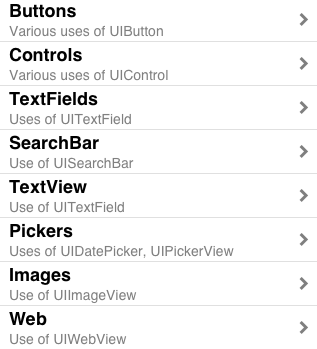
\includegraphics[width=5cm]{Toolkit/iOS/PS/TableViewSimple}
\caption{Simple Table View (list component)}
\label{TableViewSimple}
\end{center}
\end{figure}

\begin{figure}[h]
\begin{center}
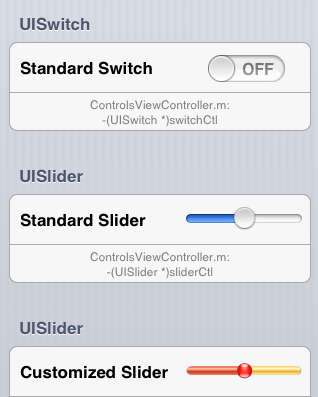
\includegraphics[width=5cm]{Toolkit/iOS/PS/TableViewGrouped}
\caption{Grouped Table View (list component)}
\label{TableViewGrouped}
\end{center}
\end{figure}



\subsubsection{Working with iOS tabbed controls}
\begin{itemize}
\item Many components in iOS \gdauts{} can be addressed as \bxname{tabbed controls} -- in a similar way to tabbed panes in a Swing \gdaut{} for example. 
\item The components \bxname{tabbed bar} and \bxname{segmented control} (\bxfigref{SegmentedControls}) are examples of two components that can be addressed with the actions on the \bxname{tabbed control} component. You can select a tab based on its content or its index, check the selection of a specific tab, check the existence etc.
\item In many cases, you will also be able to map the individual tabs as e.g. buttons or labels. As described earlier \bxpref{ToolkitiOSCorrectComponent}, we highly recommend ensuring that you are addressing the most relevant and high-level control for your test. 
\end{itemize}

\begin{figure}[h]
\begin{center}
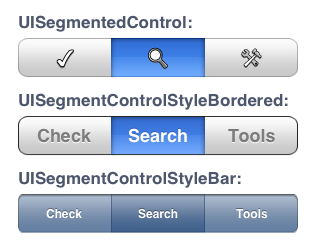
\includegraphics[width=5cm]{Toolkit/iOS/PS/SegmentedControls}
\caption{Segmented controls (tabbed controls)}
\label{SegmentedControls}
\end{center}
\end{figure}


\subsubsection{Working with iOS pickers}
\begin{itemize}
\item The iOS components \bxname{pickers} can be addressed using actions for combo components. 
\item You can select items from pickers that have only one column (\bxfigref{SinglePicker}) using the actions for \bxname{combo component} in the concrete toolkit. You can also check the existence of items in the picker, check their selection etc.
\item To work with pickers that have multiple columns, you should use the actions in the iOS toolkit to select from the picker based on the column value. In this way, you can specify which column the selection should take place in.
\end{itemize}

\begin{figure}[h]
\begin{center}
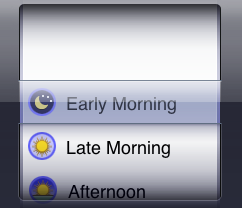
\includegraphics[width=5cm]{Toolkit/iOS/PS/SinglePicker}
\caption{Single picker (combo component)}
\label{SinglePicker}
\end{center}
\end{figure}

\begin{figure}[h]
\begin{center}
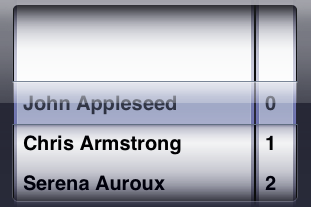
\includegraphics[width=5cm]{Toolkit/iOS/PS/MultiPicker}
\caption{Picker with multiple columns}
\label{MultiPicker}
\end{center}
\end{figure}

\textbf{Hints for working with pickers}\\
\begin{description}
\item [Check text on multi-column pickers:]{If you use the action \bxname{check text} on pickers with multiple columns, the result will be a concatenated value of all columns.}
\item [Grey items not addressable:]{Items that are grey in the picker cannot be checked or selected.}
\item [Index-based selection on infinite pickers:]{Some pickers do not have a finite amount of items -- they scroll infinitely. We strongly advise against usin index-based selection or checking on such pickers.}
\end{description}


\subsubsection{Working with gestures}
\begin{itemize}
\item In the iOS toolkit, you will find swipe actions for many components. You can use these actions to perform swipes in a specific direction.
\end{itemize}

\subsubsection{Working with the keyboard}
\label{ToolkitiOSKeyboard}
\begin{itemize}
\item To use actions such as \bxname{replace text}, you do not need to worry about using the keyboard -- the test execution component does this for you.
\item However, if you would like to press specific buttons on the keyboard such as \bxkey{DONE}, \bxkey{DELETE} and so on, then you should use the action in the \bxname{unbound\_modules\_ios} called \bxname{Tap View with Accessibility Label}.
\item This allows you to press any item on the screen (on the keyboard or elsewhere) based on its accessibility label:
\begin{itemize}
\item The accessibility label is an internal attribute for a component that is designed to be used by screen readers etc.
\item You can find out the accessibility label for an item by using the Accessibility Inspector on e.g. an iOS simulator. You can activate the Inspector via the General Settings. 
\item Once you know the label, you can enter it as a parameter (exactly as it is written).
\item Bear in mind that accessibility labels are language-dependent (i.e. you will need to translate the test data), and also sometimes orientation-dependent. It is also not necessarily the case that the accessibility label is the same as the text on the item that is visible in the \gdaut{}.  
\end{itemize}
\end{itemize}
\bxtipp{Many iOS devices have a setting activated to start each text with a capital letter. We recommend deactivating this setting for your tests, as attempts to enter lowercase text at the beginning of a textfield will otherwise fail.}

\subsubsection{Working with unmappable (unsupported) components}
If there is a component that is unsupported, then you may be able to tap it using the action in the \bxname{unbound\_modules\_ios} called \bxname{Tap View with Accessibility Label}. For more information on this action, see the section on working with the keyboard \bxpref{ToolkitiOSKeyboard}.

\subsubsection{Other important information for testing iOS \gdauts{}}
\textbf{Non-supported components}\\
The following components are not a part of the iOS toolkit, and their actions from the concrete toolkit cannot be used in iOS tests:
\begin{itemize}
\item Menus
\item Tables
\item Trees
\item Context menus
\end{itemize}

\textbf{Non-supported actions}\\
The following actions are currently not supported:
\begin{description}
\item [Restart:]{The restart action restarts the internal connection to the \gdaut{}, not the \gdaut{} itself. This means that you should consider how to reset your \gdaut{} to a known starting point as part of your \gdehandlers{} (to ensure that the test can continue despite an error). How to do this will be dependent on your \gdaut{}.}
\item [Check text on secure textfields:]{The text on a secure textfield cannot be accessed, e.g. to perform check text.}
\item [Check / store property]{ actions are not supported in the current version.}
\item [Copy to clipboard]{ is currently not supported.}
\end{description}

\textbf{Other information}\\
\begin{description}
\item [No detailed information on test failure:]{When a \gdstep{} fails, there is currently no detailed information about the reason for the error.}
\item [Support characters for text input:]{Any keys on the keyboard that are only accessible by a long press, and not by switching the whole keyboard (e.g. characters with umlauts) cannot currently be entered.}
\item [Long taps and continuous gestures:]{cannot currently be carried out.}
\item [Disabled components]{ cannot be mapped directly using e.g. tap. Instead, to collect the technical name for a disabled component, you should use the \bxname{long tap} gesture to collect all of the visible components. This includes the disabled components. }
\item [Check badge value:]{There is an action in the iOS unbound modules to let you check the text on  badges within a tab bar.}
\end{description}






